\documentclass{article}
\usepackage[utf8]{inputenc}
\usepackage[T1]{fontenc}
\usepackage{graphicx}
\usepackage{hyperref}
\usepackage{geometry}
\geometry{margin=1in}

\title{SWORD}
\date{Encyclopaedia Britannica (1771)}

\begin{document}
\maketitle

\section*{Historical source}
\textbf{Entry ID:} \texttt{entry-sword-251} \\
\textbf{Volume ID:} 191679021 \\
\textbf{Character Count:} 841

\subsection*{Extracted Text}
SWORD), an effective weapon won at the file, and fer-
ating either to eat or fish. Is parts are: the handle, geard,
and blade; to which may be added the bow, feabbard pum-
mal, \_Sraod of State,\_ which is borne before the king, lords,
and governors of counties, cities or boroughs, \&c. For
be before the King, if weights to be carried upright; the bill
as so we as the batter's wait, the blade up between the
you. For or before a dake, the blade muit decline from the head,
and be carried between the neck and the right shoulder.
For or before an sail, the blade is to the carrier between the
pouts of the shoulder and the elbow, and for or before a ba-
ros, the blade is to be borne in the head of the arm. This
determined, from no Heil denotes the digerity of a governor
than the consent let on his cost of arms.

\_Source: Filk.\_ Sec XAnsis



\section*{Source record}
\begin{itemize}
\item \textbf{Dataset:} \texttt{NationalLibraryOfScotland/encyclopaedia\_britannica\_illustrated}
\item \textbf{Dataset Revision:} \texttt{309f765b1ecc83e0a7f7762e44b4a927a7555443}
\item \textbf{Page ID:} \texttt{britannica:309f765b1ecc83e0a7f7762e44b4a927a7555443:train:251} \\
  \textbf{Filename:} \texttt{page-0251-69952e7c4a0f.jpg} \\
  \textbf{Row Index:} 251 \\
  \textbf{SHA256:} \texttt{69952e7c4a0f4026...}
\end{itemize}

\begin{figure}[h]
\centering
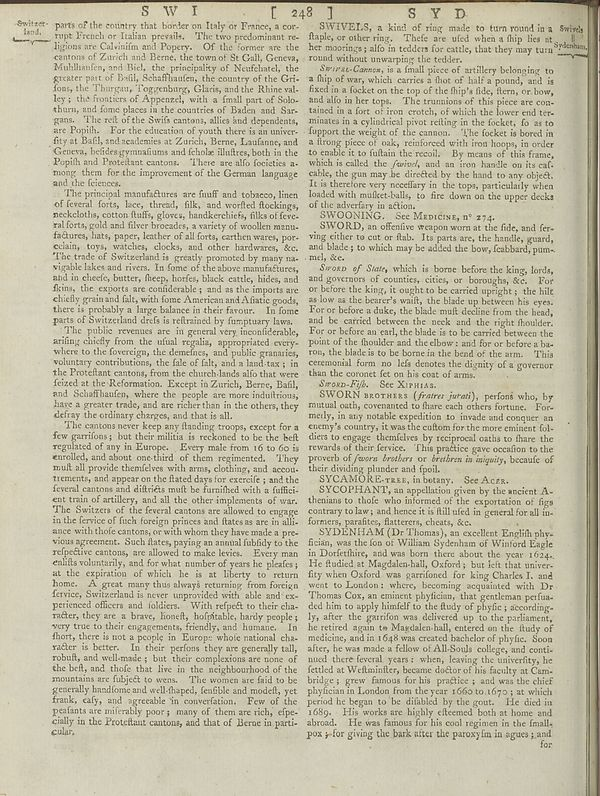
\includegraphics[width=0.85\textwidth]{../scans/page-0251-69952e7c4a0f.jpg}
\caption*{Source scan: \texttt{page-0251-69952e7c4a0f.jpg}}
\end{figure}

\end{document}
